\documentclass{article}
\usepackage[margin=1in]{geometry}
\usepackage{graphicx}
\usepackage{amsmath}
\usepackage{listings}
\usepackage{xcolor}
\usepackage{pythonhighlight}

% Define colors for code
\definecolor{bg}{rgb}{0.95,0.95,0.95}
\definecolor{comment}{rgb}{0.5,0.5,0.5}
\definecolor{keyword}{rgb}{0.25,0.5,0.75}
\definecolor{string}{rgb}{0.5,0.25,0.25}

% Set up code listings
\lstset{
    backgroundcolor=\color{bg},
    basicstyle=\ttfamily,
    commentstyle=\color{comment},
    keywordstyle=\color{keyword},
    stringstyle=\color{string},
    breaklines=true,
    frame=single,
    tabsize=4,
    captionpos=b
}

\begin{document}
\vspace{-2cm}
\title{\LARGE \textbf{TRINITY COLLEGE DUBLIN} \\ % Reduce the space between the title and the next line
\large School of Computer Science and Statistics}
\author{Abhishek Zade}
\date{} % Optionally remove date if not needed
\maketitle
\vspace{-1cm} % Adjust this value to reduce space between the author and title

\noindent
\textbf{StudentId:} 24332461 \hfill \textbf{Dataset id:} 5--10-5 \\
\textbf{Week 2 Assignment \hfill CS7CS4/CSU44061 Machine Learning} \\

% Horizontal line
\noindent\rule{\textwidth}{0.4pt} % This creates a horizontal line across the width of the page

\section*{Model Solution}

\subsection*{(a)}
\begin{enumerate}
    \item[(i)]   
The scatter plot displays data points spread out on a graph with $X_1$ and $X_2$ as the axes, both ranging from -1 to 1. The two classes seem to be separated along the $X_2$ axis. The +1 class, shown as dark green + markers, is mainly located in the upper half of the plot for $X_2$ values greater than about 0.25, while the -1 class, represented by dark blue dots, mostly occupies the lower half of the plot with $X_2$ values less than 0.5. The plot suggests that there might be a relatively simple decision rule to effectively classify these points, possibly by using a threshold on the $X_2$ value to separate the two classes.\\
    \begin{center}
        \centering
        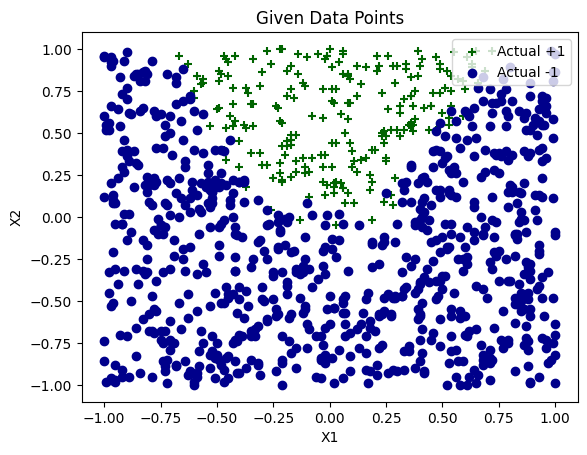
\includegraphics[width=0.75\linewidth]{final_a_1.1.png}
        \centering \\
        \captionof{Figure}{\centering (1.1)}
        \label{fig:enter-label}
    \end{center}

    \newpage
    \item[(ii)] \textbf{Total Features in model: 2} \\
\textbf{Classes: [-1, 1]} \\
\textbf{Intercept:} -2.249 \\
\textbf{Coefficient for Feature $X_1$:} 0.177 \\
\textbf{Coefficient for Feature $X_2$:} 3.652 \\

From the following data, it is clear that Feature $X_2$ has more weight than Feature $X_1$. We can say that Feature $X_2$ is more important in predicting $Y$. Now, the question arises: why does $X_2$ have more importance? When training a model in scikit-learn, one of the ways the logistic regression algorithm determines the optimal weights for features is by analyzing their relationships with the output. This includes metrics like the correlation between the feature and the output, as well as the variance of the feature. Correlation measures the strength and direction of a linear relationship between two variables, while variance measures how spread out the values are. \\

\textbf{Correlation between X1 and Y:} 0.014 \\
\textbf{Correlation between X2 and Y:} 0.571 \\
\textbf{Variance of X1:} 0.343 \\
\textbf{Variance of X2:} 0.337 \\

To calculate these metrics, I used numpy.var to calculate the variance and numpy.corr to calculate the correlation. After analyzing the output, we can see that while $X_1$ and $X_2$ have similar variance, $X_2$ shows a much higher correlation with $Y$ (0.571 for $X_2$ compared to 0.014 for $X_1$). This explains why $X_2$ has a larger coefficient and thus, more influence on predicting $Y$. Therefore, $X_2$ is the more important feature in the model. Using numpy.var and numpy.corr helped quantify these relationships, making it easier to understand why $X_2$ has a greater impact. This analysis ensures that the model is interpretable and that feature importance is accurately determined. \\   
    \item[(iii)] 
     \textbf{Model:} Logistic Regression \\

     \begin{center}
        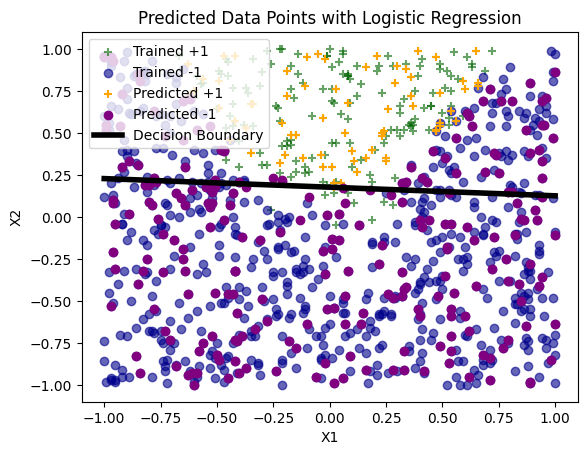
\includegraphics[width=0.75\linewidth]{a.1.2.1.png} \\
                \centering
    \captionof{Figure}{\centering (1.2)} % Center the caption
    \end{center} \\
    
    The following figure(1.2) represents Actual vs. Predicted Data Points using Logistic Regression with the Decision Boundary. To draw the decision boundary, I used the line equation as follows: \(\text{coef}[0] \cdot X_1 + \text{coef}[1] \cdot X_2 + \text{intercept} = 0\). The code first calculates the minimum and maximum values of the feature \(X_1\) to establish its range. It sets the number of points to 50 and computes the step size to generate evenly spaced \(X_1\) values within this range. Using a list comprehension, it creates a list of \(X_1\) values from the minimum to the maximum. Subsequently, it calculates the corresponding \(X_2\) values for each \(X_1\) using the rearranged line equation, expressed as \(X_2 = -\frac{\text{coef}[0]}{\text{coef}[1]} \cdot X_1 - \frac{\text{intercept}}{\text{coef}[1]}\). This equation illustrates the linear relationship defined by the logistic regression model, resulting in the \(X_2\) values that visually represent the decision boundary separating different predicted classes in the dataset. \\

    
    \item[(iv)] The model's predictions demonstrate a clear alignment with the training data, particularly in areas where \(X_2\) plays a significant role. The decision boundary, shown as a nearly horizontal line, reflects the fact that \(X_2\) has a much higher coefficient (3.65) compared to \(X_1\) (0.18), indicating that \(X_2\) is the dominant feature influencing the classification. This is supported by the strong correlation between \(X_2\) and the target variable \(Y\) (0.57), while \(X_1\) shows minimal correlation (0.01). The model performs well in classifying points where \(X_2\) has high or low values. For instance, data points with higher \(X_2\) values (above the decision boundary) are predominantly classified as class `+1`, while those with lower \(X_2\) values (below the boundary) are classified as class `-1`. However, some misclassifications are evident, especially near the decision boundary, where points from both classes are intermixed. In these regions, orange `+1` predictions overlap with purple `-1` training points, and vice versa, showing the model's difficulty in perfectly separating the two classes. The predictions are fairly reliable but not perfect, and the decision boundary effectively captures the overall structure of the data.
\end{enumerate}
\subsection*{(b)}
\begin{enumerate}
\item[(i)] \\
\begin{table}[h!]
    \centering
    \begin{tabular}{|c|c|c|c|}
        \hline
        C Value & Intercept & Coefficient of $X_1$ & Coefficient of $X_2$ \\ \hline
        0.001 & -0.281 & 0.006 & 0.269 \\ \hline
        0.01 & -0.376 & 0.048 & 0.780 \\ \hline
        1.0 & -0.142 & 0.109 & 2.994 \\ \hline
        42.78 & 0.027 & 0.268 & 5.707 \\ \hline
        55.776 & 0.032 & 0.273 & 5.817 \\ \hline
        57.21 & 0.034 & 0.274 & 5.819 \\ \hline
        82.337 & 0.040 & 0.277 & 5.911 \\ \hline
        87.867 & 0.040 & 0.278 & 5.925 \\ \hline
        98.948 & 0.043 & 0.281 & 5.984 \\ \hline
    \end{tabular}
    \caption{Intercept and Coefficients for Different Values of C}
\end{table}
The above table presents different parameter values for the LinearSVM model. The \textbf{C Value} represents the regularization parameter that controls the model complexity. A higher C value reduces the regularization effect, allowing the model to fit the data more closely. The \textbf{Intercept} is the bias term of the model, while the \textbf{Coefficients of $X_1$ and $X_2$} represent the weights assigned to the respective features. As the value of C increases, both coefficients and the intercept tend to increase, indicating stronger relationships with the features.
\newpage
\item[(ii)] \\
\textbf{Model:} LinearSVM Model \\

\begin{center}
    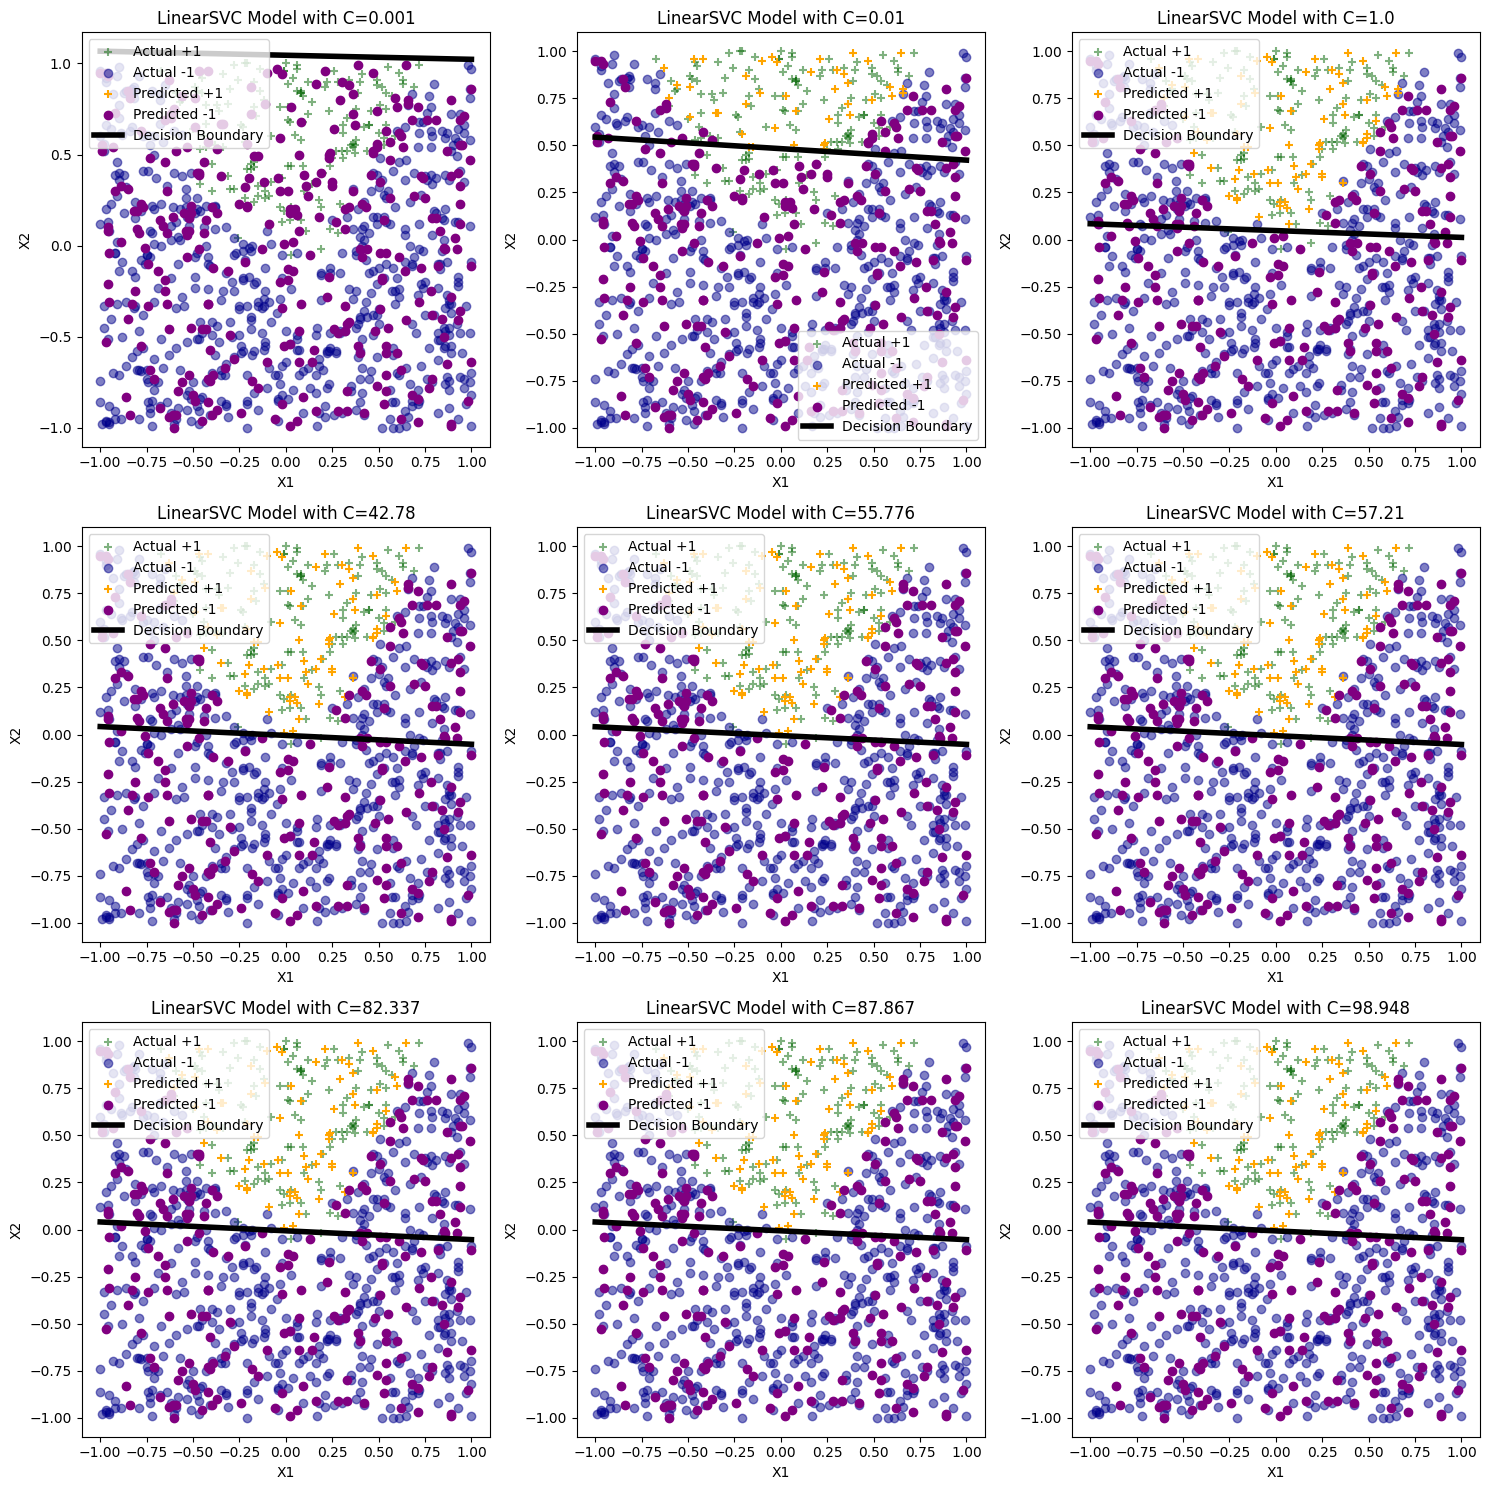
\includegraphics[width=1\linewidth]{fin_b1.1.png}
    \centering
    \caption{Fig}{\centering (2.1)}
    \label{fig:enter-label}
\end{center}
  \\
     The Fig (2.1) displays several subplots showing SVM (Support Vector Machine) classifiers trained with different values of the regularisation parameter $C$. Each subplot visualises the decision boundary (black line), actual data points (dark green + for class +1 and dark blue O for class -1), and the model's predictions (orange for predicted +1 and dark purple for predicted -1). \\

    \item[(iii)] The regularization parameter $C$ in an SVM model controls how the model balances between having a larger margin and making fewer classification errors. When $C$ is small (like $C$=0.001), the model focuses on creating a wider margin, even if it misclassifies some points. This results in lower coefficient values and a simpler decision boundary. As $C$ increases (like $C$=1 $C$=0.1 $C$=100), the model becomes stricter about minimizing classification errors, leading to higher coefficients and a more complex boundary.

    \item[(iv)] The Logistic Regression model gives much more weight to Feature $X_2$, with a large coefficient of 3.65, and less to Feature $X_1$ (0.1778). In contrast, the SVC model keeps the feature weights more balanced, such as \( X_1 = 0.07752 \) and \( X_2 = 1.38152 \) for \( C = 82.337 \), meaning it recognizes the importance of $X_2$ but not as strongly as Logistic Regression. The intercept (bias) for Logistic Regression is larger at -2.25, compared to SVC, which has intercepts around -0.81. The larger intercept and stronger weight on $X_2$ in Logistic Regression suggest that it draws a steeper decision boundary, making it better at separating the data based on the features. SVC, with its more regularized and balanced feature weights, creates a more even decision boundary, but this might cause it to underemphasize the key feature, $X_2$. Overall, Logistic Regression's higher emphasis on the more important feature ($X_2$) gives it an edge in classification effectiveness.
\end{enumerate}

\subsection*{(c)}
\begin{enumerate}
    \item[(i)] 
    \textbf{Intercept:} -0.861 \\
    \textbf{Coefficient for Feature $X_1$:} 0.249 \\
    \textbf{Coefficient for Feature $X_2$:} 4.868 \\ 
    \textbf{Coefficient for Feature $X_3$:} -6.878 \\
    \textbf{Coefficient for Feature $X_4$:} 0.369 \\

    \item[(ii)] The new Logistic Regression model, which now includes the original features \( X_1 \) and \( X_2 \) along with their squared terms (\( X_1^2 \) and \( X_2^2 \)), shows significantly improved performance. The coefficient for \( X_2 \) (4.87) is larger compared to the previous Logistic Regression model (3.65), further emphasizing the importance of \( X_2 \) in predicting the target. The coefficient for \( X_1 \) (0.25) is also slightly higher than in the earlier model (0.18). Additionally, the coefficients for the newly introduced features are as follows: Coefficient for Feature \( X_3 \) (squared term of \( X_1 \)): -6.878, and Coefficient for Feature \( X_4 \) (squared term of \( X_2 \)): 0.369. The main improvement comes from the inclusion of the squared terms, which allow the model to capture non-linear relationships in the data. Squaring the features enables the model to account for more complex patterns, such as curved decision boundaries, which a purely linear model might miss. This added flexibility helps the model fit the data more accurately, including the ability to predict non-linear points effectively, thereby reducing errors and leading to significantly improved predictions.
    \begin{center}
         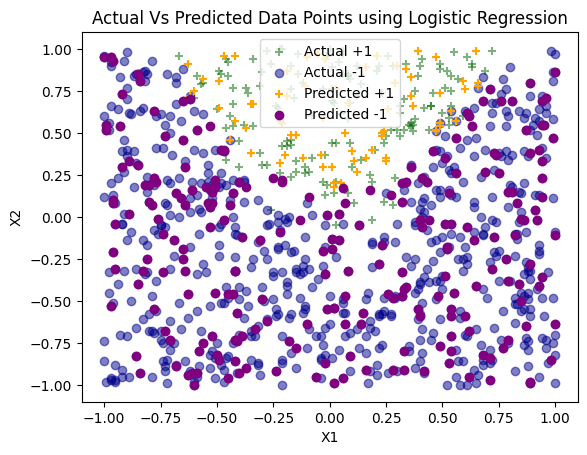
\includegraphics[width=0.75\linewidth]{final_c_1.1.png}
         \centering
        \captionof{Figure}{\centering (3.1)}
    \end{center}

    \item[(iii)] \textbf{Baseline Accuracy:} 0.775 \\
\textbf{Classifier Accuracy:} 0.97 \\

The results indicate that the baseline accuracy is 0.775, meaning that a simple model that always predicts the most common class would achieve 77.5\% correct predictions. In contrast, your classifier attained an accuracy of 0.97, which is a significant improvement of 19.5 percentage points. This suggests that our classifier is effectively learning useful patterns from the data. The substantial increase in accuracy indicates that the model has a strong capacity to generalize and make correct predictions beyond what a naive approach could achieve.


    \item[(iv)] 
    \textbf{Decision Boundary for Logistic Regression Model} \\
    \begin{center}
        \centering
        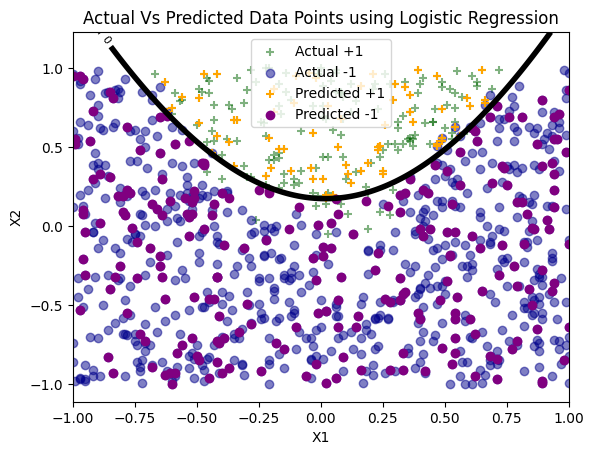
\includegraphics[width=0.75\linewidth]{Final_c_1.3.png} \\
        \centering
        \captionof{Figure}{\centering (3.2)}
    \end{center}
    \\
    In Figure 3.2, a contour plot is generated for a decision boundary in a four-feature space, incorporating both original features \(X_1\) and \(X_2\), along with their squared terms \(X_3 = X_1^2\) and \(X_4 = X_2^2\). The decision boundary can be represented by the equation:

\[
Z = \text{intercept} + \text{coef}[0] \cdot X_1 + \text{coef}[1] \cdot X_2 + \text{coef}[2] \cdot X_3 + \text{coef}[3] \cdot X_4
\]

where \(\text{coef}[0]\), \(\text{coef}[1]\), \(\text{coef}[2]\), and \(\text{coef}[3]\) are the coefficients for the features. The code first calculates the minimum and maximum values of \(X_1\) and \(X_2\) to define the grid. Next, it generates values for \(X_1\) and computes corresponding values for \(X_2\) based on a derived linear equation. A meshgrid is created using \texttt{np.meshgrid} to evaluate the decision boundary over the specified range. The contour lines are plotted to visualize the decision regions, aiding in understanding how the model classifies the feature space based on the learned coefficients.
\end{enumerate}

\newpage
\section*{Apendix}

\begin{python}
import numpy as np
import pandas as pd
import matplotlib.pyplot as plt
from sklearn.model_selection import train_test_split
from sklearn.linear_model import LogisticRegression
from sklearn.svm import LinearSVC
from sklearn import metrics

# id:5--10-5 
df = pd.read_csv("./data/week2.csv")
X1 = df.iloc[:, 0]
X2 = df.iloc[:, 1]
Y = df.iloc[:, 2]
X = np.column_stack((X1,X2))
y = np.array(Y)
df.dropna(inplace = True)

postive = [i for i in range(len(y)) if y[i] == 1]
plt.scatter([X[i][0] for i in postive], [X[i][1] for i in postive], marker='+', color='darkgreen', label='Actual +1')

negative = [i for i in range(len(y)) if y[i] == -1]
plt.scatter([X[i][0] for i in negative], [X[i][1] for i in negative], marker='o', color='darkblue', label='Actual -1')

plt.xlabel('X1')
plt.ylabel('X2')
plt.legend()
plt.title('Given Data Points')
plt.show()

X_train, X_test, y_train, y_test = train_test_split(X, y, test_size=0.30, random_state=42)
log_reg = LogisticRegression()
log_reg.fit(X_train, y_train)
classes_ = log_reg.classes_
coef = log_reg.coef_[0]
intercept = log_reg.intercept_[0] 
features_in = log_reg.n_features_in_

print(f"Total Features in model: {log_reg.n_features_in_}")
print(f"classes: {classes_}")
print(f"Intercept: {round(intercept,3)}")
print(f"Coefficient for Feature X1: {round(coef[0],3)}")
print(f"Coefficient for Feature X2: {round(coef[1],3)}")

data = {
    'X1' : X1,
    'X2' : X2,
    'Y' : Y
}
dataFrame = pd.DataFrame(data)
corr_X1_Y = dataFrame['X1'].corr(dataFrame['Y'])
corr_X2_Y = dataFrame['X2'].corr(dataFrame['Y'])
print(f"Correlation between X1 and Y: {round(corr_X1_Y,3)}")
print(f"Correlation between X2 and Y: {round(corr_X2_Y,3)}")
variance_X1 = np.var(X1, ddof=1)
variance_X2 = np.var(X2, ddof=1)
print(f'Variance of X1: {round(variance_X1,3)}')
print(f'Variance of X2: {round(variance_X2,3)}')

y_pred = log_reg.predict(X_test)

positive = [i for i in range(len(y)) if y[i] == 1]
plt.scatter([X[i][0] for i in positive], [X[i][1] for i in positive], marker='+', color='darkgreen', label='Actual +1', alpha=0.6)

negative = [i for i in range(len(y)) if y[i] == -1]
plt.scatter([X[i][0] for i in negative], [X[i][1] for i in negative], marker='o', color='darkblue', label='Actual -1', alpha=0.6)

positive_pred = [i for i in range(len(y_pred)) if y_pred[i] == 1]
plt.scatter([X_test[i][0] for i in positive_pred], [X_test[i][1] for i in positive_pred], marker='+', color='orange', label='Predicted +1', alpha=1)

negative_pred = [i for i in range(len(y_pred)) if y_pred[i] == -1]
plt.scatter([X_test[i][0] for i in negative_pred], [X_test[i][1] for i in negative_pred], marker='o', color='purple', label='Predicted -1', alpha=1)


min_X1 = min(X1)
max_X1 = max(X1)

num_points = 50
step_size = (max_X1 - min_X1) / (num_points - 1)

x1_vals = [min_X1 + i * step_size for i in range(num_points)]
x2_vals = [ -((coef[0] * x) / coef[1]) - (intercept / coef[1]) for x in x1_vals]

plt.plot(x1_vals, x2_vals, color='black', label='Decision Boundary', linewidth=4)

plt.xlabel('X1')
plt.ylabel('X2')
plt.legend()
plt.title('Actual Vs Predicted Data Points using Logistic Regression')
plt.show()

C = [8.2337e+01, 5.5776e+01, 8.7867e+01, 4.2780e+01, 5.7210e+01, 9.8948e+01, 1.0000e-03 , 1.0000e-02, 1.0000e+00]
C.sort()
n_cols = 3
n_rows = (len(C) + n_cols - 1) // n_cols
fig, axs = plt.subplots(n_rows, n_cols, figsize=(15, n_rows * 5))
axs = axs.flatten()


for i in range(len(C)):
    
    Linear_svc = LinearSVC(C = C[i])
    Linear_svc.fit(X_train, y_train)
    coef = Linear_svc.coef_[0]
    intercept = Linear_svc.intercept_[0]
    print(" ")
    print(f"Intercept for C={C[i]} : {round(intercept,3)}")
    print(f"Coefficient of X1 for C={C[i]} : {round(coef[0],3)}")
    print(f"Coefficient of X2 for C={C[i]} : {round(coef[1],3)}")

    y_pred = Linear_svc.predict(X_test)
    positive = [i for i in range(len(y_train)) if y_train[i] == 1]
    negative = [i for i in range(len(y_train)) if y_train[i] == -1]
    axs[i].scatter([X_train[i][0] for i in positive], [X_train[i][1] for i in positive], 
                     marker='+', color='darkgreen', label='Actual +1',alpha=0.5)
    axs[i].scatter([X_train[i][0] for i in negative], [X_train[i][1] for i in negative], 
                     marker='o', color='darkblue', label='Actual -1',alpha=0.5)

    positive_pred = [i for i in range(len(y_pred)) if y_pred[i] == 1]
    negative_pred = [i for i in range(len(y_pred)) if y_pred[i] == -1]
    axs[i].scatter([X_test[i][0] for i in positive_pred], [X_test[i][1] for i in positive_pred], 
                     marker='+', color='orange', label='Predicted +1',alpha=1)
    axs[i].scatter([X_test[i][0] for i in negative_pred], [X_test[i][1] for i in negative_pred], 
                     marker='o', color='purple', label='Predicted -1',alpha=1)


    min_X1 = min(X1)
    max_X1 = max(X1)

    num_points = 50
    step_size = (max_X1 - min_X1) / (num_points - 1)

    x1_vals = [min_X1 + i * step_size for i in range(num_points)]
    x2_vals = [ -((coef[0] * x) / coef[1]) - (intercept / coef[1]) for x in x1_vals]

    axs[i].plot(x1_vals, x2_vals, color='black', label='Decision Boundary',linewidth=4)
    
    axs[i].set_title(f"LinearSVC Model with C={C[i]}")
    axs[i].set_xlabel('X1')
    axs[i].set_ylabel('X2')
    axs[i].legend()

plt.tight_layout()
plt.show()

X3 = (X1 ** 2).astype(str).to_numpy()
X4 = (X2 ** 2).astype(str).to_numpy()
X = np.column_stack((X1,X2,X3,X4))

X_train, X_test, y_train, y_test = train_test_split(X, y, test_size=0.30, random_state=42)
log_reg = LogisticRegression()
log_reg.fit(X_train, y_train)
coef = log_reg.coef_[0]
intercept = log_reg.intercept_[0] 

print(f"Intercept: {round(intercept,3)}")
print(f"Coefficient for Feature X1: {round(coef[0],3)}")
print(f"Coefficient for Feature X2: {round(coef[1],3)}")
print(f"Coefficient for Feature X3: {round(coef[2],3)}")
print(f"Coefficient for Feature X4: {round(coef[3],3)}")

y_pred = log_reg.predict(X_test)

postive = [i for i in range(len(y)) if y[i] == 1]
plt.scatter([X[i][0] for i in postive], [X[i][1] for i in postive], marker='+', color='darkgreen', label='Actual +1',alpha=0.5)

negative = [i for i in range(len(y)) if y[i] == -1]
plt.scatter([X[i][0] for i in negative], [X[i][1] for i in negative], marker='o', color='darkblue', label='Actual -1',alpha=0.5)

positive_pred = [i for i in range(len(y_pred)) if y_pred[i] == 1]
plt.scatter([X_test[i][0] for i in positive_pred], [X_test[i][1] for i in positive_pred], marker='+', color='orange', label='Predicted +1', alpha=1)

negative_pred = [i for i in range(len(y_pred)) if y_pred[i] == -1]
plt.scatter([X_test[i][0] for i in negative_pred], [X_test[i][1] for i in negative_pred], marker='o', color='purple', label='Predicted -1', alpha=1)


min_X1, max_X1 = np.min(X1), np.max(X1)
min_X2, max_X2 = np.min(X2), np.max(X2)

num_points = 500
step_size = (max_X1 - min_X1) / (num_points - 1)

x1_vals = [min_X1 + i * step_size for i in range(num_points)]
x2_vals = [ -((coef[0] * x) / coef[1]) - (intercept / coef[1]) for x in x1_vals]

extended_min_X2 = min(x2_vals) - 1
extended_max_X2 = max(x2_vals) + 1

X1_grid, X2_grid = np.meshgrid(x1_vals, np.linspace(extended_min_X2, extended_max_X2, num_points))

X3_grid = X1_grid ** 2
X4_grid = X2_grid ** 2

Z = intercept + coef[0] * X1_grid + coef[1] * X2_grid + coef[2] * X3_grid + coef[3] * X4_grid
contours = plt.contour(X1_grid, X2_grid, Z, levels=[0], colors='black', linewidths=4)
plt.clabel(contours, inline=True, fontsize=8)

plt.xlabel('X1')
plt.ylabel('X2')
plt.legend()
plt.title('Actual Vs Predicted Data Points using Logistic Regression')
plt.show()

classifier_prediction = log_reg.predict(X_train)
classifier_accuracy = metrics.accuracy_score(y_train,classifier_prediction)

y_test_unique, y_test_frequency = np.unique(y_test, return_counts=True)
max_frequency_index = np.argmax(y_test_frequency)
y_pred_baseline = np.full((len(y), 1), y_test_unique[max_frequency_index])
baseline_accuracy = metrics.accuracy_score(y,y_pred_baseline)

print(f"Baseline Accuracy: {round(baseline_accuracy,3)}")
print(f"Classifier Accuracy: {round(classifier_accuracy,3)}")



\end{python}

\end{document}